\section{Modelado de prote\'{i}nas por predicci\'{o}n de contactos} \label{contactosPred}

Las matrices de contactos (ver secci\'{o}n \ref{estr34})  han sido durante mucho tiempo una fuente de inspiraci\'{o}n de m\'{e}todos 
de predicci\'{o}n estructural, con la idea subyacente de 'si somos capaces de predecir con informaci\'{o}n evolutiva qu\'{e} residuos de 
una secuencia contactan, entonces podremos resolver su estructura' \citep{Gobel1994,deJuan2013}.

La informaci\'{o}n evolutiva en cuesti\'{o}n es normalmente un alineamiento m\'{u}ltiple de secuencias hom\'{o}logas, que se espera
capturen de forma impl\'{i}cita las limitaciones que impone la estructura terciaria de un dominio a las sustituciones de amino\'{a}cidos
que contactan. La funci\'{o}n matem\'{a}tica que se emplea habitualmente para estudiar esto es la 
\htmladdnormallink{informaci\'{o}n mutua}{http://es.wikipedia.org/wiki/Informaci\%C3\%B3n\_mutua} (MI), 
que mide la dependencia entre dos variables, en este caso columnas de un alineamiento.

\begin{figure}
\begin{center} 
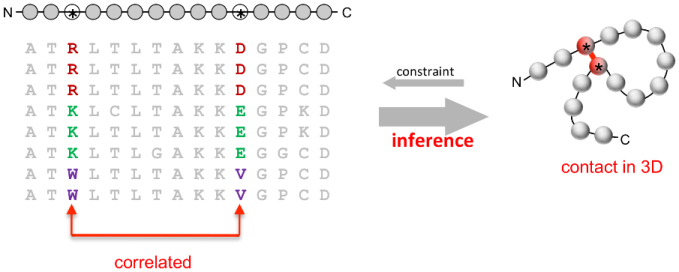
\includegraphics{EVfoldcorr}
\caption%[]
{
Las mutaciones correlacionadas entre columnas de un alineamiento m\'{u}ltiple se pueden emplear para predecir contactos entre residuos en el plegamiento.
Figura tomada de \cite{Marks2011} y reproducida con permiso de los autores.
}
\label{fig:EVfold1}
\end{center}
\end{figure}

Por tanto, el problema de la predicci\'{o}n de contactos se puede plantear as\'{i}:
\begin{itemize}
\item \textbf{PROBLEMA:} conocemos la secuencia de una prote\'{i}na y las de muchas secuencias hom\'{o}logas
\item \textbf{SOLUCI\'{O}N PROPUESTA:} alineamos las secuencias, buscamos posiciones que muestren evidencia de coevoluci\'{o}n 
y buscamos plegamientos compatibles con esos contactos
\end{itemize}

El algoritmo \htmladdnormallink{EVfold}{http://EVfold.org} %, publicado originalmente en \citep{Marks2011}, 
emplea estos elementos
para hacer predicciones de contactos de alta calidad, ya que es capaz de distinguir entre posiciones de la secuencia
que directamente contactan (causativas) de las que correlacionan simplemente porque contactan con un mismo residuo (transitivas). 
Usando su terminolog\'{i}a,
MI es un modelo local de probabilidad de contactos, que ellos son capaces de corregir y convertir en un modelo global usando conceptos 
de la mec\'{a}nica estad\'{i}stica y la maximizaci\'{o}n de la entrop\'{i}a. El modelo global se llama de Informaci\'{o}n Directa (DI)
\citep{Marks2011}.

\begin{figure}
\begin{center} 
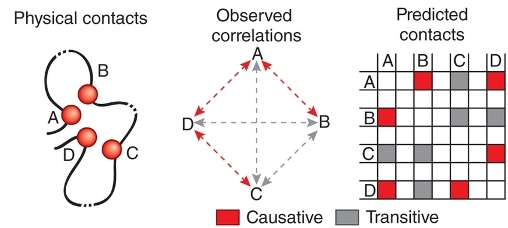
\includegraphics{EVfold22}
\caption%[]
{
Definici\'{o}n de contactos entre residuos (A,B,C,D) y de correlaciones directas y transitivas.
Figura tomada de \cite{Marks2012}. Copyright (2012) Nature Biotechnology.
}
\label{fig:EVfold1.1}
\end{center}
\end{figure} %https://www.ncbi.nlm.nih.gov/pmc/articles/PMC4319528/figure/F2/

\begin{figure}
\begin{center} 
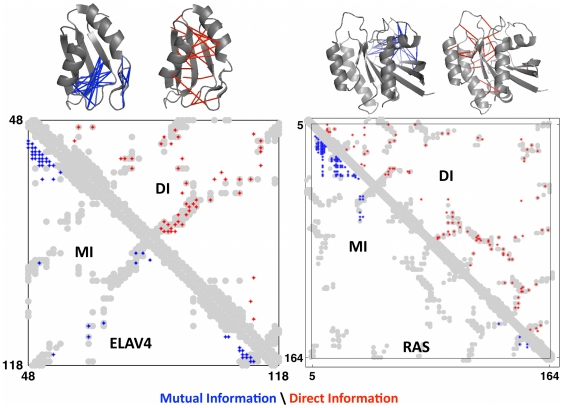
\includegraphics{EVfold3}
\caption%[]
{
La inferencia de contactos entre residuos es mejor con el modelo global (DI, ver texto) que con el modelo local MI.
La figura muestra predicciones de contactos para las prote\'{i}nas ELAV4 (derecha) y RAS (izquierda).
Las predicciones globales se reparten uniformemente por la secuencia y se solapan mejor con los contactos observados en estructuras experimentales.
Figura tomada de \cite{Marks2011} y reproducida con permiso de los autores.
}
\label{fig:EVfold2}
\end{center}
\end{figure}

La siguiente figura muestra el diagrama de flujo completo del m\'{e}todo \htmladdnormallink{EVfold}{http://EVfold.org}, 
que ha sido posteriormente adaptado para prote\'{i}nas transmembrana \citep{Hopf2012} y 
tambi\'{e}n para complejos cuaternarios \citep{Hopf2014}:

\begin{figure}
\begin{center} 
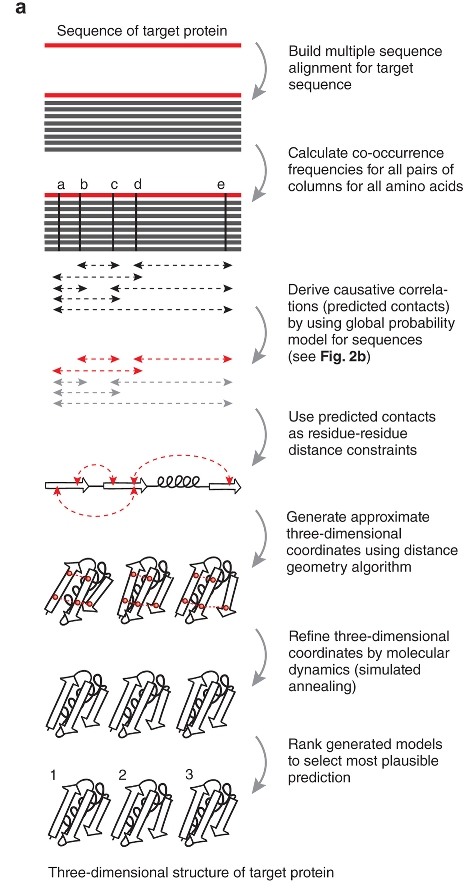
\includegraphics{EVfold21}
\caption%[]
{
Algoritmo de plegamiento de prote\'{i}nas en base a observaciones de mutaciones correlacionadas,
que se transforman en predicciones de contactos, tomado de \cite{Marks2012}. Copyright (2012) Nature Biotechnology.
}
\label{fig:EVfold3} %https://www.ncbi.nlm.nih.gov/pmc/articles/PMC4319528/figure/F2/
\end{center}
\end{figure}

La siguiente figura muestra los resultados de un experimento de validaci\'{o}n de EVfold:

\begin{figure}
\begin{center} 
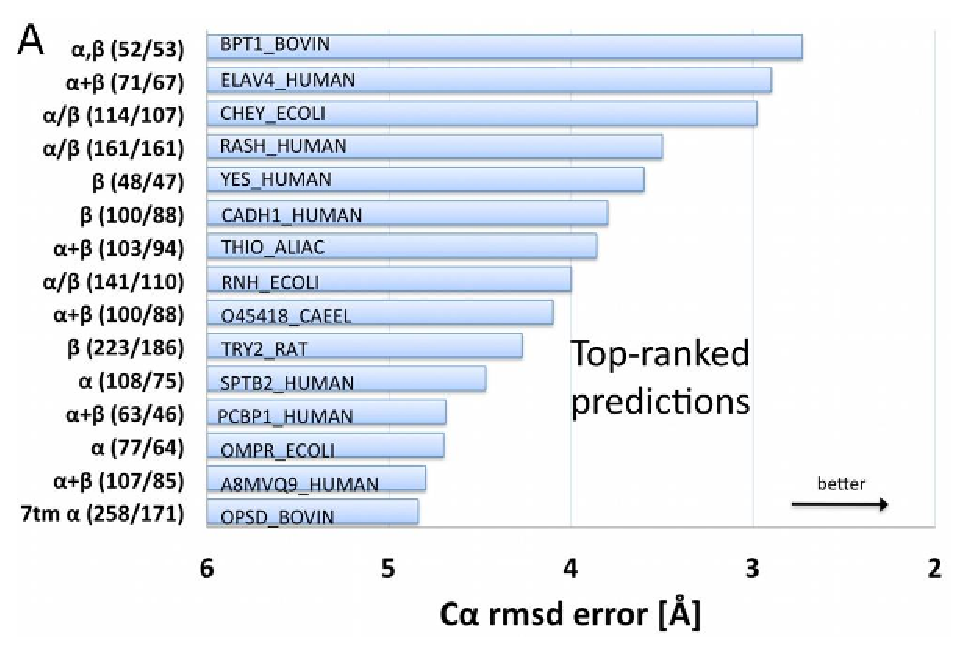
\includegraphics{EVfoldbenchA}
\caption%[]
{
Calidad de las mejores predicciones de EVfold en un conjunto de 15 prote\'{i}nas con diferentes composiciones de estructuras secundaria.
Entre par\'{e}ntesis se muestran el n\'{u}mero de residuos del dominio modelado y 
el n\'{u}mero de residuos sobre los que se calcul\'{o} el RMSD entre el modelo y la estructura experimental.
Figura tomada de \cite{Marks2011} y reproducida con permiso de los autores.
}
\label{fig:EVfold4}
\end{center}
\end{figure}

Esta familia de m\'{e}todos  se est\'{a} desarrollando todav\'{i}a y sigue habiendo avances importantes \citep{Buchan2017}.
El m\'{a}s notable es que el uso de secuencias metagen\'{o}micas permite ampliar el universo de secuencias lo suficiente 
para mejorar las predicciones de contactos (usando por ejemplo \htmladdnormallink{GREMLIN}{http://gremlin.bakerlab.org/submit.php}) 
y obtener as\'{i} estructuras, de momento bacterianas, de numerosos plegamientos desconocidos \citep{Ovchinnikov2017}. 
Adem\'{a}s, \citet{Ovchinnikov2017} proponen una funci\'{o}n para estimar la calidad de los modelos si hay suficientes secuencias para abordar
este tipo de modelado:

\begin{equation}
N_{f} = \frac{clusters_{nr80}}{\sqrt L} 
\end{equation} 

En esta funci\'{o}n el numerador representa el total de clusters de secuencias hom\'{o}logas no redundantes al 80\% 
encontradas con \htmladdnormallink{HHblits}{https://toolkit.tuebingen.mpg.de/#/tools/hhblits} y el numerador es la longitud de la secuencia problema. 
Cuando $N_{f} > 64$ se obtienen modelos de buena calidad. 
 
Para poner en pr\'{a}ctica estos algoritmos se puede realizar el siguiente ejercicio:

\begin{itemize}

\item Visita \htmladdnormallink{UniProt}{http://www.uniprot.org/}, elige una prote\'{i}na y extrae su secuencia S.

\item Busca secuencias similares a S y gu\'{a}rdalas en un archivo.

\item Calcula un alineamiento m\'{u}ltiple A que incluya a S con sus hom\'{o}logos, elimina las secuencias muy cortas y 
guarda el resultado en un fichero FASTA.

\item Con ayuda de los 
\htmladdnormallink{m\'{e}todos suplementarios}{https://doi.org/10.1371/journal.pone.0028766.s017} de \cite{Marks2011}
modifica el c\'{o}digo fuente del programa 3.4 para calcular el peso de las secuencias en base a su identidad
y sumar pseudoconteos y de esa manera calcular con mayor precisi\'{o}n MI en tu alineamiento A.
Hay tambi\'{e}n c\'{o}digo fuente disponible en 
\htmladdnormallink{http://evfold.org/evfold-web/code.do}{http://evfold.org/evfold-web/code.do}.

\item Construye un modelo 3D para S.

\item Edita el archivo PDB del modelo y marca algunas parejas de residuos con valores altos de MI. Para ello puedes usar la columna del factor B,
dejando a '00.00' el resto de residuos. 

\item Visualiza el modelo editado y discute los resultados obtenidos.

\end{itemize}

\verbatiminput{code/prog3.4.pl}

